\documentclass[12pt,oneside]{fithesis2}
\usepackage[slovak]{babel}       % Multilingual support
\usepackage[utf8]{inputenc}       % UTF-8 encoding
\usepackage[T1]{fontenc}          % T1 font encoding
\usepackage[                      % A sans serif font that blends well with Palatino
  scaled=0.86
]{berasans}
\usepackage[                      % A tt font if you do not like LM's tt
  scaled=1.03
]{inconsolata}
\usepackage[                      % Clickable links
  plainpages = false,               % We have multiple page numberings
  pdfpagelabels                     % Generate pdf page labels
]{hyperref}
\usepackage{blindtext}            % Lorem ipsum generator
\usepackage{amsmath}

\thesislang{sk}                   % The language of the thesis
\thesistitle{Vyhľadávanie najbližších vektorov s využitím knižnice FLANN}       % The title of the thesis
\thesissubtitle{Bakalárska práca}  % The type of the thesis
\thesisstudent{Tomáš Durčák}          % Your name
\thesiswoman{false}                % Your gender
\thesisfaculty{fi}                % Your faculty
\thesisyear{Jar \the\year}     % The academic term of your thesis defense
\thesisadvisor{RNDr. David Novák, Ph.D.}   % Your advisor

\begin{document}
  \FrontMatter                    % The front matter
    \ThesisTitlePage                % The title page
    \begin{ThesisDeclaration}       % The declaration
      \DeclarationText
      \AdvisorName
    \end{ThesisDeclaration}
    \begin{ThesisThanks}            % The acknowledgements (optional)
      I would like to thank my supervisor\,\dots
    \end{ThesisThanks}
    \begin{ThesisAbstract}          % The abstract
      The aim of the bachelor work is to provide\,\dots
    \end{ThesisAbstract}
    \begin{ThesisKeyWords}          % The keywords
      keyword1, keyword2\,\dots
    \end{ThesisKeyWords}
    \tableofcontents                % The table of contents
%   \listoftables                   % The list of tables (optional)
%   \listoffigures                  % The list of figures (optional)
  
  \MainMatter                     % The main matter
    \chapter{Úvod}          % Chapters
    \Blindtext
    \chapter{Základné pojmy}
    
    	\section{Vektorový priestor}
    Vektorový priestor $ \Omega = D_1D_2. . .D_n $ má dimenziu $n$. Objekt (resp. vektor, resp.bod)  $\mathcal{O} = [a_1, a_2, . . . , a_n] $ patriaci do vektorového priestoru je jednoznačne určeny svojimi súradnicami $ a_i \in D_i, 1 \le i \le n, $ ktorých je práve $n$. Každá jednotlivá dimenzia má svoju doménu $D_i$ - množinu hodnôt (resp. vlastností), ktoré môže prislušná vektorová súradnica nadobúdať.
    	
    Vektorový priestor $\Omega$, definujeme nad určitým polom $\mathbf{P} $, s význačným prvkom $\mathbf{0}$ a dvomi binárnymi operáciami, sčítaním $+ : \Omega \times \Omega \rightarrow \Omega $  a násobením $. : \mathbf{P}  \times \Omega \rightarrow \Omega$, takými že platí: 
     
\begin{equation*}
\forall u,v,w \in \Omega : (u + v)+w = u+(v+w) 
\end{equation*}
\begin{equation*}
\exists\mathbf{0} \in \Omega : u+\mathbf{0} = \mathbf{0}+u = u
\end{equation*}
\begin{equation*}
\forall u \in \Omega \; \exists \; u \in \Omega : u+(-u)  = \mathbf{0}
\end{equation*}
\begin{equation*}
\forall a,b \in \mathbf{P} \; \exists \; u \in \Omega : (a.b).u = a.(b.u) 
\end{equation*}
\begin{equation*}
\forall u \in \Omega : 1.u=u  \textrm{ kde } 1 \in \mathbf{P}  \textrm{ je jednotkový prvok z } \mathbf{P} 
\end{equation*}
\begin{equation*}
\forall a,b \in \mathbf{P} \; \exists \;u \in \Omega : (a+b).u = a.u + b.u 
\end{equation*}
\begin{equation*}
\forall a \in \mathbf{P} \; \exists \;u,v \in \Omega : a.(u+v) = a.u + a.v 
\end{equation*} \\
\textbf{Poznámka:} Vektorový podpriestor je tiež vektorový priestor.

\begin{figure}
  \centering
  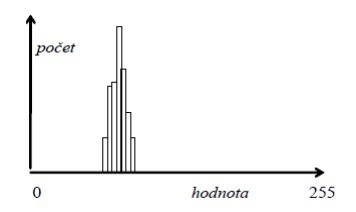
\includegraphics[width=6cm]{gis_histogram_obrazu.png}
  \caption{Histogram farieb so siedmimi farebnými odtieňmi.}
  \label{fig:triangle}
\end{figure}  

\textbf{Príklad:}
Obrázok (resp. jeho histogram farieb) može byť vektorom vo vektorovom priestore a mať súradnice podľa počtu pixelov z každého farebného odtieňu.
Potom vektor z histogramu farieb je:
\begin{equation}
\{(\alpha_1,\beta_1),...(\alpha_M,\beta_M)\}
\end{equation}
kde $M$ je počet farebných odtieňov. \\
Iným príkladom môže byť dokument reprezentovaný ako
vektor v $m$-rozmernom priestore príznakov, ktoré zodpovedajú jednotlivým slovám – tzv.termom. Množina $n$ dokumentov je reprezentovaná ako matica $n\times m$. Neplnovýznamové slová (pomocne slovesá, spojky...) sa zvyčajne odstránia.


    \section{Metrický priestor}
    
    Metrický priestor je množina, na ktorej je definovaná vzdialenosť pre všetky prvky z množiny. Táto vzdialenosť sa nazýva metrika. Metriku môžme definovať ako funkciu, ktorá určuje vzdialenosť medzi dvomi objektami. \\ \\
    \textbf{Definícia:} Nech $X\neq 0$ je množina. Definujme zobrazenie $d: X \times X \rightarrow R $, ktoré spĺňa nasledujúce vlastnosti:
    \begin{align*}
    \textrm{ Pre všetky } x,y,z \in X \qquad d(x,x) &= 0 \\
    d(x,y) &\textgreater 0 \qquad x\neq y \\
    d(x,y) &= d(y,x) \\
    d(x,z) + d(z,y) &\geq d(x,y)
    \end{align*}
    
    Množinu \textbf{$X$} nazývame \textbf{základnou množinou}, zobrazenie $d$ \textbf{metrikou} a usporiadanu dvojicu $(X,d)$ \textbf{metrickým priestorom}.
    V tej istej množine možme definovať rôzne metriky. Metrika $d$ musí byť vždy nezáporná. \\ \\
    \textbf{Príklad:} 
    Vzdialenosť dvoch bodov na priamke v $ \mathbf{R} \quad d=|x-y| $ alebo v rovine v
     $\mathbf{R} \quad d = \sqrt{(x_1-y_1)^2+(x_2-y_2)^2}$.
    

    
    \chapter{Knižnica Flann}
    	\section{Podkapi}
    	\section{Podkapitola}
    	\paragraph{dsdsd}

    
    \chapter{Výsledky testov}
    
    \chapter{Záver}
    \appendix
    \chapter{First appendix}        % Appendices
    \Blindtext
    \chapter{Another appendix}
    \Blindtext
    % Bibliography goes here
    % Index goes here (optional)
\end{document}
